\section{Methodology}

The whole idea behind VOYO is based on a hybrid-deterministic thesis: Using a
delegate-to-solver contract, which explicitly prevents our LLM model from ever allowing
feasibility, geography, and even numerical optimisation. The architecture of our system will be
discussed in our methodology chapter, a discussion of our contracts will be completed and the
role and purpose of each of our engines will be explained to our entire system. We will also take
you on a walkthrough of an ablation protocol, where we systematically remove components of
our system, and elucidate whether or not they are actually important in real-world context. We
will present our ablation protocol to demonstrate our approach of tying an LLM to a deterministic
solver yields finer results, as opposed to the LLM doing everything on its own — making our
argument scientifically, not just theoretically, true. Structures of both what is trusted to be done
by the components and engines, and what is explicitly prohibited from being done by the
components and engines, will also be shown.


\subsection{System Architecture: A Four Layer Hybrid}

There are four layers involved with VOYO's system architecture: a Presentation Layer, a Gateway
Layer, an Agentic Orchestration Layer, and finally a Ground Truth Data Layer. The design
principle that ties them together is the \textbf{curate$\rightarrow$optimise split}: a system where
the LLM reasons and curates, while the deterministic system verifies and optimises. This is
accurately represented in Figure~\ref{fig:voyo_architecture}, which shows the full system
architecture. The mobile client layer is a thin presentation layer, and processes such as
orchestration, state management, and data verification run against a 310-POI database.

\begin{figure}[h]
    \centering
    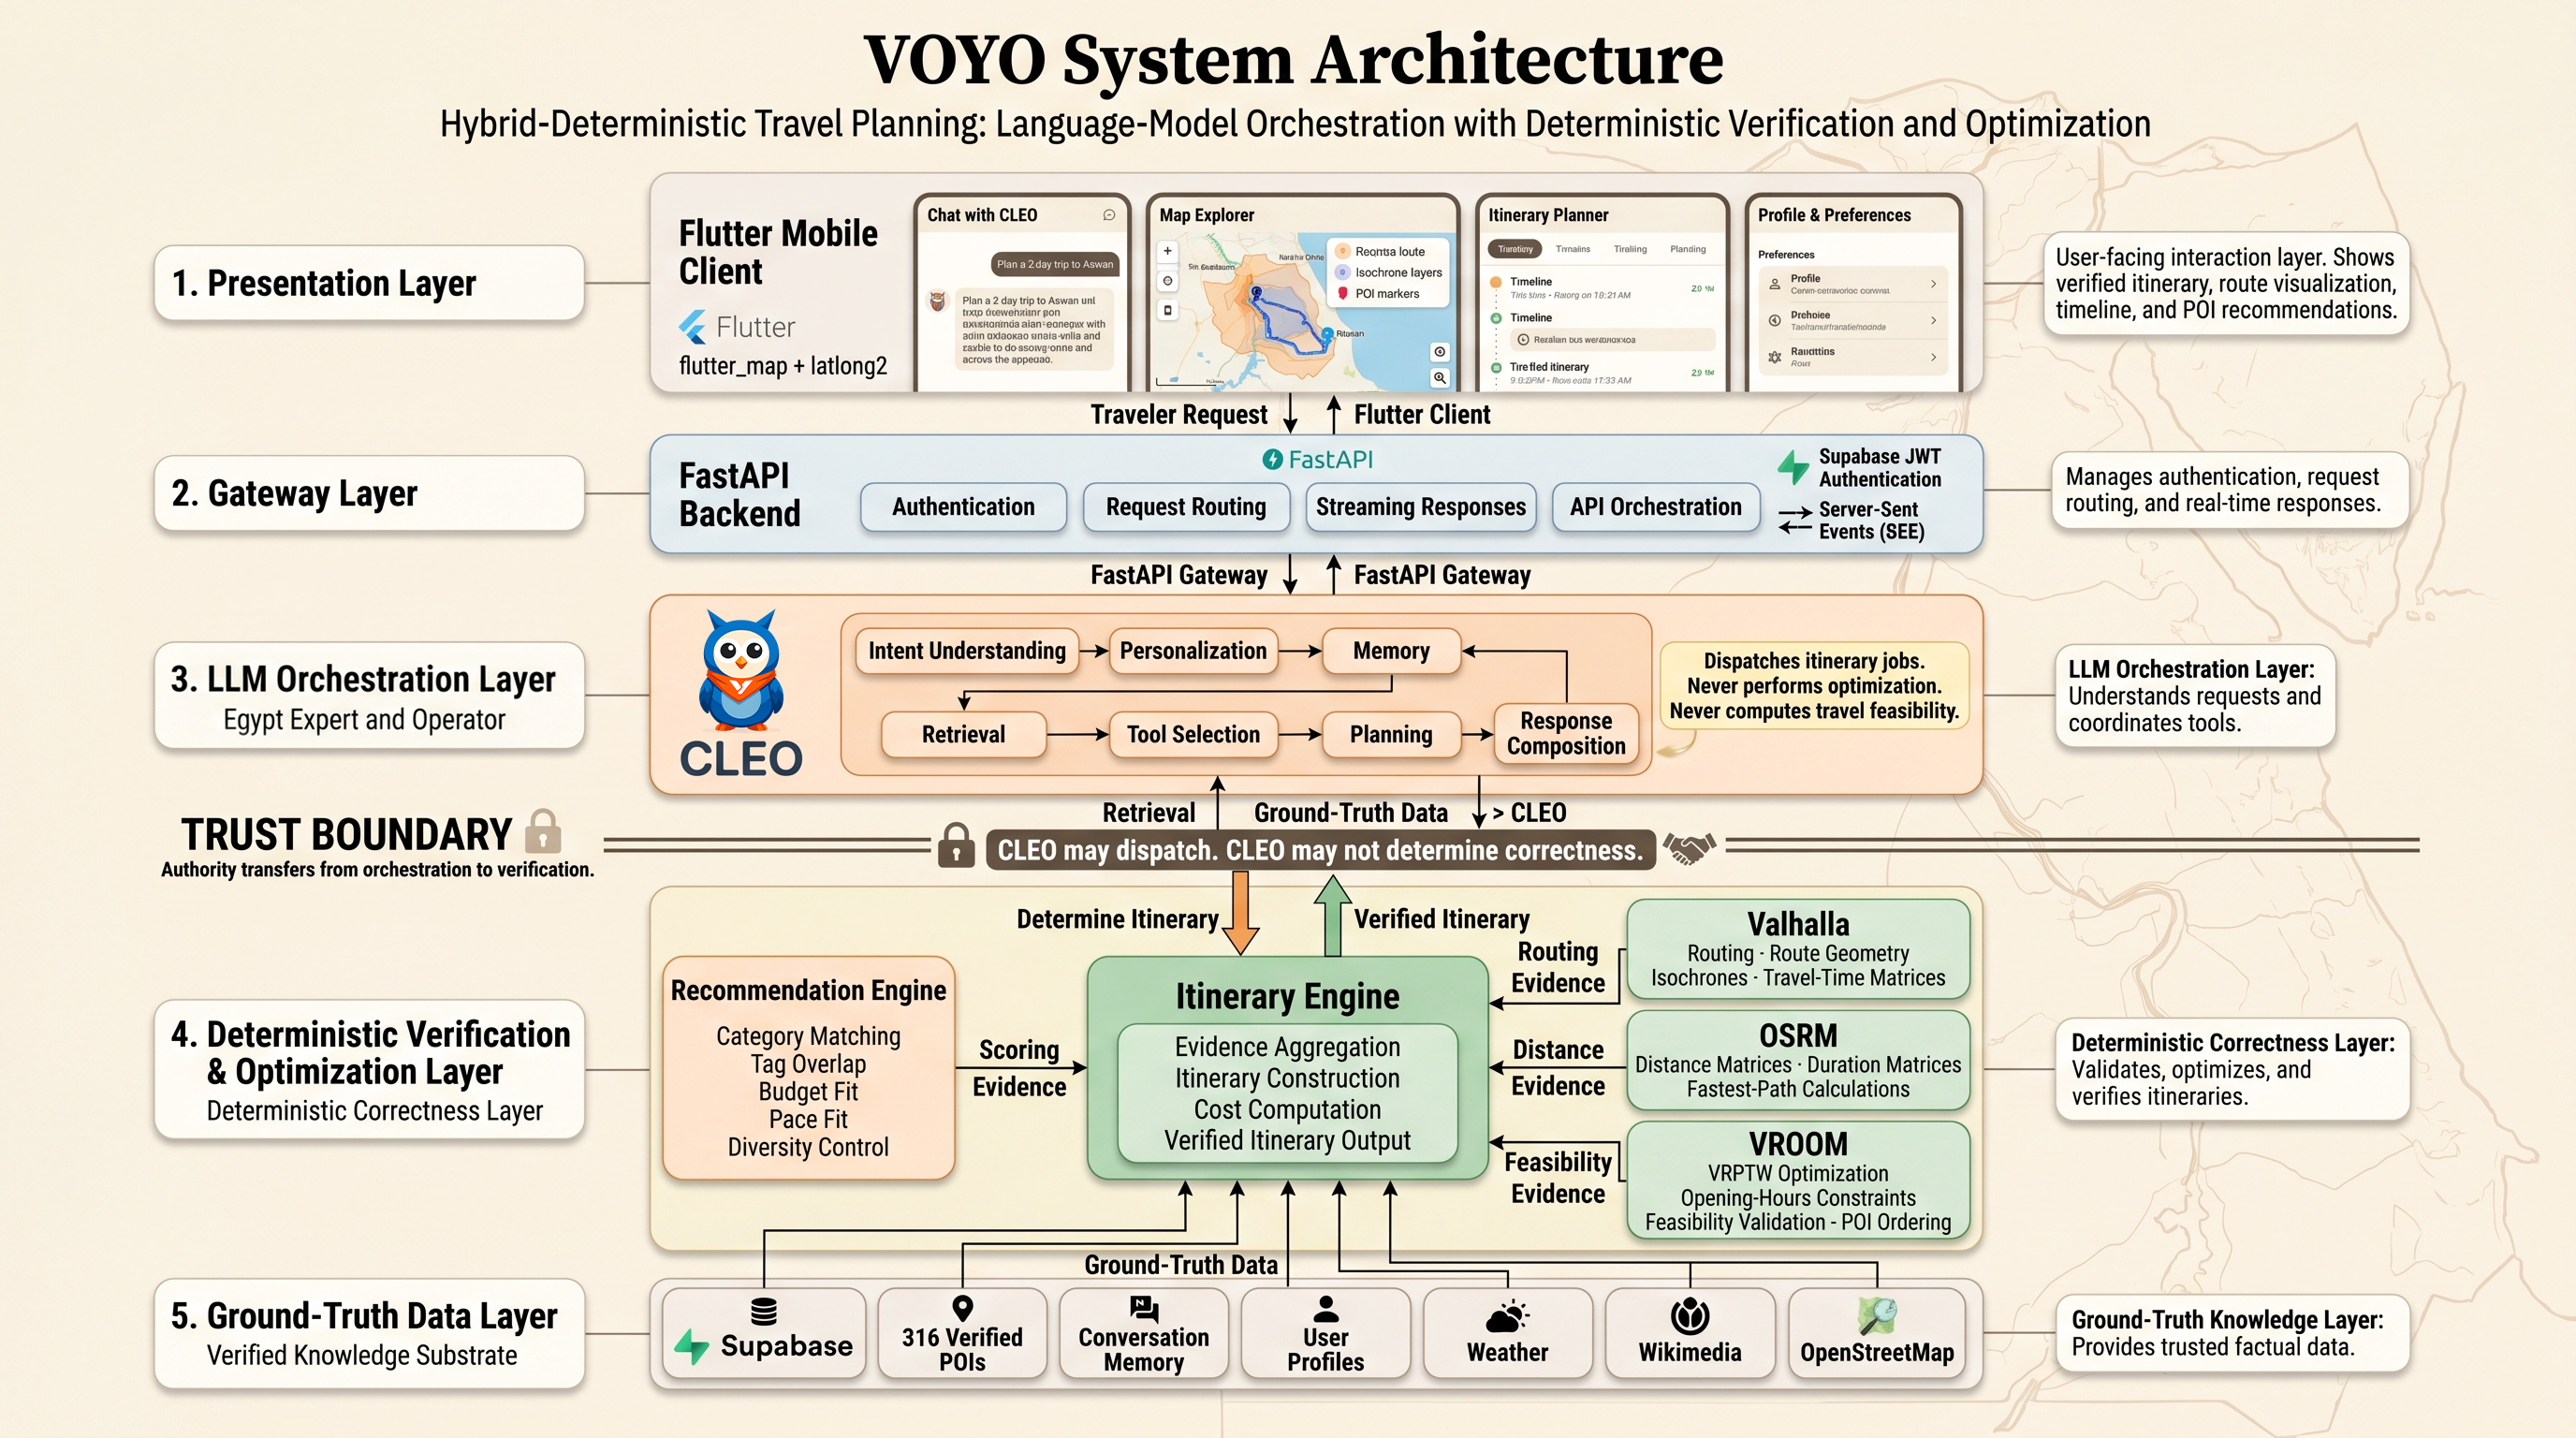
\includegraphics[width=\textwidth]{../figures/VOYO_FINAL_System_Architecture.png}
    \caption{VOYO System Architecture: Hybrid-Deterministic Travel Planning with
             Language-Model Orchestration and Deterministic Verification and Optimisation.}
    \label{fig:voyo_architecture}
\end{figure}

This unique split exists because LLM planning has a proven failure record. Tang et al.\ note that
``Pure LLMs cannot refer to specific POI lists, resulting in outdated or hallucinated POIs''
\cite[§1, p.~1]{itinera_tang_2024} and that ``LLMs lack the optimisation capabilities required for
planning tasks, leading to suboptimal itineraries'' \cite[§1, p.~1]{itinera_tang_2024}, which can
be circuitous, lack detail, and include impractical information. Today's LLMs simply do not
perform well in certain situations — calculating distances, ordering stops along a route, checking
opening hours, and verifying time feasibility — which is why we developed a deterministic engine
specifically designed to handle those cases. The LLM is used purely for understanding queries in
natural language and for composing answers in natural language.

Wang et al.'s blueprint decomposes agentic behaviour into four key modules: a profiling module,
a memory module, a planning module, and an action module, where ``the profiling module impacts
the memory and planning modules, and collectively, these three modules influence the action
module'' \cite[§2.1]{wang_agent_survey}. CLEO's architecture is inspired by the one used by Wu
et al.\ in their AutoGen framework, in which a conversational LLM is separated from a
deterministic tool. ``AutoGen agents are customizable, conversable, and can operate in various
modes that employ combinations of LLMs, human inputs, and tools'' \cite[Abstract]{autogen}.
Conversation held between multiple agents is what keeps the LLM structurally off the
feasibility path \cite[§1]{autogen}.


\subsection{CLEO Conversational Layer}

CLEO (Cairo's Local Expert and Operator) is VOYO's LLM intent layer. It aims to achieve three
objectives as efficiently and accurately as possible: it parses natural-language user requests,
stores preference and memory state based on the user profile and the settings the user selects
upon each itinerary generation, and lastly composes a readable human response. As stated, it
never attempts to reason about geography, feasibility, or numerical optimisation.

CLEO's structure is inspired by the four-module blueprint of Wang et al.\ \cite[§2.1]{wang_agent_survey}:
a profile module which gathers data from the user's travel preferences (identified through a
series of questions upon logging in, and again when building each itinerary); a memory module
which consists of conversation history backed by Supabase (\texttt{conversation\_memory.py});
and a planning module which operates using a ReAct loop. On the LLM side of the trust boundary
table in §3.6, CLEO is permitted three jobs: intent parsing (figuring out what the user actually
wants to do), preference maintenance (recalling and updating what the user actually prefers),
and response composition (presenting the results of our deterministic engines in a
human-readable form).

Within our system, we have also implemented a grounding policy to prevent CLEO from
answering certain user queries using only the LLM's training memory. To achieve this, a
per-iteration \texttt{force\_tool} policy is applied via \texttt{\_classify\_response\_style}. User
queries classified as \texttt{detailed} enforce a \texttt{search\_pois} call before any response
is formed. More general POI queries (\texttt{standard}) force any tool call, ruling out pure
memory answers. More general queries (\texttt{concise}) leave tool use as \texttt{auto}. This
process alone consumes a sub-optimal number of tokens, which is why tool results are
immediately passed through \texttt{\_slim\_for\_llm}, which summarises results into eight
distinct fields — reducing token use approximately eight-fold.

We verified offline that the following operations work correctly: POI queries trigger a tool call;
itinerary queries trigger \texttt{search\_pois} specifically; and POI name resolution
(\texttt{\_resolve\_poi\_id}) accurately translates name strings to database integer identifiers.
Locations already identified in a previous tool call are recognised and returned unchanged,
because resolving what has already been resolved is redundant. Upon inevitable unrecognised
inputs (a place not in the database, misspelled locations, and so on), the system does not
crash — it returns a value the rest of the code can handle safely.

CLEO has two types of tools: retrieval and dispatch. Retrieval tools fetch information;
dispatch tools hand off tasks to other engines. Our retrieval tools, \texttt{search\_pois} and
\texttt{get\_poi\_details}, operate over our 310-POI database using a three-tier
\texttt{ilike} search. The first tier searches for a direct name or address match. The second tier
searches inside longer text fields such as POI descriptions, when the first tier does not return
enough results. The third tier applies category and region filtering, falling back to broader
categories such as ``Islamic Architecture'' or regions such as ``Old Cairo'' when tiers one and
two cannot find what is needed. In addition, we have included supporting tools that aid trip
planning: a tool that fetches real-time weather, a tool that stores user preferences, and a tool
that fetches high-quality POI images from Wikimedia. The \texttt{curate\_itinerary} handler
dispatches to \texttt{src/itinerary/engine.py} and does not compute the itinerary itself. When
CLEO detects a query requiring a full itinerary, it packages the request and passes it to the
dedicated itinerary engine rather than building one itself. We chose SQL as our database
search mechanism because every result is explainable — you can pinpoint exactly which fields
match which terms, making retrieval deterministic. In our context this transparency was more
valuable than the marginal quality boost offered by vector embeddings or BM25, because our
system is built on verified data and a strict trust boundary.


\subsection{The Delegate-to-Solver Contract}

The LLM may dispatch requests to the deterministic engines but may never produce feasibility
assessments, geographical optimisations, or numerical optimisations. The individual
prohibitions correspond to specific failure modes documented by \citeauthor{itinera_tang_2024}
and \citeauthor{travelplanner} for LLM-alone baselines.

\textbf{The negative specification.} CLEO is not permitted to: (a) calculate the time or distance
between POIs; (b) determine whether a series of POIs can be visited within a day's time budget;
(c) validate opening-hours compliance; (d) order POIs along a route; (e) produce any numerical
value — price, distance, duration, latitude, longitude — except by relaying a value fetched from
the verified database or returned by a deterministic engine. These are precisely the operations
that ``LLMs lack the optimisation capabilities required for planning tasks''
\cite[§1, p.~1]{itinera_tang_2024}. \citeauthor{travelplanner} quantify the failure independently:
GPT-4 achieves a 0.6\% success rate on constrained travel planning without deterministic
support \cite{travelplanner} — not just a failure, but an almost complete failure.

\textbf{The positive specification.} The contract's positive form is equally simple: CLEO may
dispatch to the deterministic engines but may never compute their outputs. The
\texttt{curate\_itinerary} handler creates the request, which is then presented to
\texttt{src/itinerary/engine.py}; the engine in turn delegates time-window feasibility computation
to VROOM and distance matrix computation to Valhalla/OSRM. The LLM never occupies the
feasibility or optimisation path.

\textbf{Auditability.} A blacklist is only effective if it can be verified. The trust boundary table in
§3.6 contains one row for each class of computation, specifying which side of the boundary it
belongs to and citing the source that warrants that assignment. The ablation protocol in §3.5
goes one step further, registering a configuration in which the contract is intentionally violated —
the only way to know whether the contract actually makes a difference.
